\section{Parallel Design}

\subsection{Serial VGLCS Algorithm}
\begin{frame}
	\frametitle{Serial VGLCS Algorithm}
	\begin{figure}
		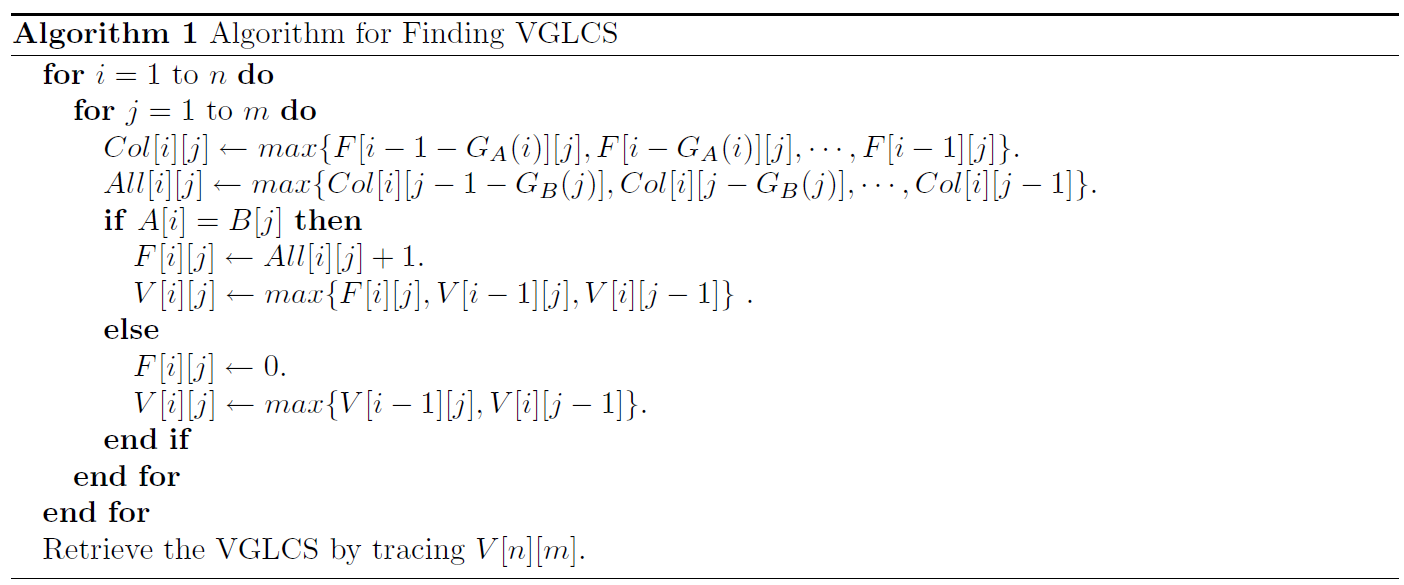
\includegraphics[scale=0.3]{figure/fig-VGLCS-algo.png}
	\end{figure}
\end{frame}

\subsection{Data Structure}
\begin{frame}
    \frametitle{Data Structure}
    \begin{itemize}
    \setlength\itemsep{1em}
    	\item Incremental Suffix Maximum Query
    		\begin{itemize}
    			\setlength\itemsep{1em}
    			\item Binary Indexed Tree (Fenwick Tree): $\mathcal{O}(\log n)$
    			\item Segment Tree: $\mathcal{O}(\log n)$
    			\item Van Emde Boas Tree: $\mathcal{O}(\log \log n)$
    			\item Disjoint Set: $\Omega(\alpha(n))$
    			\item Sparse Table: $\mathcal{O}(n \log n)$ -- $\mathcal{O}(1)$
    		\end{itemize}
    	\item Which one is cache-friendly/ exploit parallelism easily?
    \end{itemize}
\end{frame}

\subsection{Hybrid Stages}
\begin{frame}
	\frametitle{Data Dependency}
	\begin{itemize}
		\setlength\itemsep{1em}
		\item We want to remove \texttt{All[i][j]} because its data dependency 
			is hard to parallel.
		\item The $O(n \log n)$ -- $O(1)$ sparse table is a good alternative plan. 
		\item However, parallel algorithm will be $O(n^2 \max(\log n, \alpha(n)) / p + n \max(\log n, \alpha(n)))$ 
			with $p$ processors.
	\end{itemize}
\end{frame}

\begin{frame}
	\frametitle{Parallel VGLCS Algorithm}
\end{frame}

\begin{frame}
	\frametitle{Workload Imbalance}
	\begin{itemize}
		\setlength\itemsep{1em}
		\item Disjoint set has a lot of indirect jumps, and it leads cache miss penatly.
		\item Due to the compensatory hardware threading and L2 cache layout, affinity 
			is important on the MIC. We can control of thread affinity via \tt{KMP\_AFFINITY}
	\end{itemize}
\end{frame}

\begin{frame}
	\frametitle{Improve Workload (TODO)}
	\begin{itemize}
		\setlength\itemsep{1em}
		\item Reduce cache miss
			\begin{itemize}
				\setlength\itemsep{1em}
			 	\item Relayout data of disjoint set: structure of array, 
			 		array of structure, hybrid combinations, or ...
			 	\item Software caches
			 	\item Data compression
			\end{itemize}
		\item Reduce indirect jumps
			\begin{itemize}
				\setlength\itemsep{1em}
				\item The policy of path compression / union by rank
			\end{itemize}
	\end{itemize}
\end{frame}

\begin{frame}
	\frametitle{Exploit Parallelism (TODO)}
	\begin{itemize}
		\setlength\itemsep{1em}
		\item Using rank convergence in dynamic programming algorithm
			\footnote{Paper: Efficient Parallelization Using Rank Convergence in 
				Dynamic Programming Algorithm}
		\item Simultaneously, it reduces memory usage on a single processor,
			less cache miss penalty will be faster(?).
	\end{itemize}
\end{frame}

\subsection{Serial part-VG LCS Algorithm (TODO)}
\begin{frame}
	\frametitle{Serial part-VG LCS Algorithm}
\end{frame}

\subsection{Parallel part-VG LCS Algorithm (TODO)}
\begin{frame}
	\frametitle{Parallel part-VG LCS Algorithm}
\end{frame}

\subsection{Optimization (TODO)}
\begin{frame}
	\frametitle{Optimization (TODO)}
	\begin{itemize}
		\setlength\itemsep{1em}
		\item Coalesced memory access or memory coalescing
			\begin{itemize}
				\item Doubling algorithm creates smaller table
					and uses more computation in query.
			\end{itemize}
		\item Loop fission / fusion: improve data locality, 
			but maybe increase thread overhead.
	\end{itemize}
\end{frame}